\subsection{Vector Displays}
A vector display/monitor displays graphics by drawing from point to point.
Vector displays utilize \gls{crt} technology, which contain one or more electron emitters that fire electron beams that are deflected onto a phosphorescent screen to display images.

The basic vector display is monochromatic.
However, certain displays with colour support exist.
Figure \ref{fig:color_crt} shows how it works.
By using a shadow mask - that is a perforated plate that acts as a filter - between the electron guns and the screen, different colours can be displayed.
This is achieved by having one electron gun for red, green and blue.
Each gun shoots electron at different angles through the mask, and different intensities for each gun can create different colours. \cite{monitors}

\begin{figure}
	\centering
	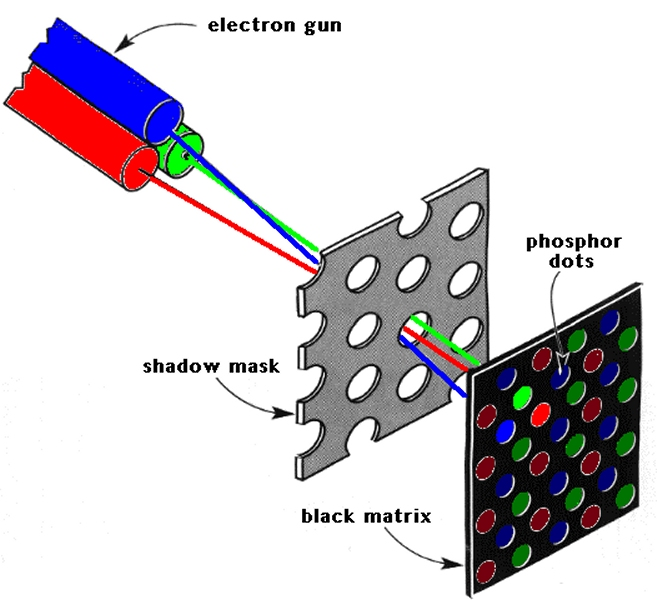
\includegraphics[width=0.5 \textwidth]{images/color_crt.jpg}
	\caption{Dot phosphor in coloured \gls{crt} \cite{monitors}}
	\label{fig:color_crt}
\end{figure}

Vector displays are pretty much obsolete today, because of raster screens' inexpensiveness and support for graphics with a higher level of detail.\cite{lcd-vs-crt}
Also, vector graphics can - with modern algorithms - efficiently be translated to raster graphics, called rasterisation.
Translating raster graphics to vector graphics, or vectorisation, is possible, but for highly detailed images, it results in a significant loss of quality \cite{vectorisation}.
